\documentclass{beamer}\usepackage[]{graphicx}\usepackage[]{color}
%% maxwidth is the original width if it is less than linewidth
%% otherwise use linewidth (to make sure the graphics do not exceed the margin)
\makeatletter
\def\maxwidth{ %
  \ifdim\Gin@nat@width>\linewidth
    \linewidth
  \else
    \Gin@nat@width
  \fi
}
\makeatother

\definecolor{fgcolor}{rgb}{0.345, 0.345, 0.345}
\newcommand{\hlnum}[1]{\textcolor[rgb]{0.686,0.059,0.569}{#1}}%
\newcommand{\hlstr}[1]{\textcolor[rgb]{0.192,0.494,0.8}{#1}}%
\newcommand{\hlcom}[1]{\textcolor[rgb]{0.678,0.584,0.686}{\textit{#1}}}%
\newcommand{\hlopt}[1]{\textcolor[rgb]{0,0,0}{#1}}%
\newcommand{\hlstd}[1]{\textcolor[rgb]{0.345,0.345,0.345}{#1}}%
\newcommand{\hlkwa}[1]{\textcolor[rgb]{0.161,0.373,0.58}{\textbf{#1}}}%
\newcommand{\hlkwb}[1]{\textcolor[rgb]{0.69,0.353,0.396}{#1}}%
\newcommand{\hlkwc}[1]{\textcolor[rgb]{0.333,0.667,0.333}{#1}}%
\newcommand{\hlkwd}[1]{\textcolor[rgb]{0.737,0.353,0.396}{\textbf{#1}}}%
\let\hlipl\hlkwb

\usepackage{framed}
\makeatletter
\newenvironment{kframe}{%
 \def\at@end@of@kframe{}%
 \ifinner\ifhmode%
  \def\at@end@of@kframe{\end{minipage}}%
  \begin{minipage}{\columnwidth}%
 \fi\fi%
 \def\FrameCommand##1{\hskip\@totalleftmargin \hskip-\fboxsep
 \colorbox{shadecolor}{##1}\hskip-\fboxsep
     % There is no \\@totalrightmargin, so:
     \hskip-\linewidth \hskip-\@totalleftmargin \hskip\columnwidth}%
 \MakeFramed {\advance\hsize-\width
   \@totalleftmargin\z@ \linewidth\hsize
   \@setminipage}}%
 {\par\unskip\endMakeFramed%
 \at@end@of@kframe}
\makeatother

\definecolor{shadecolor}{rgb}{.97, .97, .97}
\definecolor{messagecolor}{rgb}{0, 0, 0}
\definecolor{warningcolor}{rgb}{1, 0, 1}
\definecolor{errorcolor}{rgb}{1, 0, 0}
\newenvironment{knitrout}{}{} % an empty environment to be redefined in TeX

\usepackage{alltt}
\IfFileExists{upquote.sty}{\usepackage{upquote}}{}
\begin{document}

\title{Wordcloud}
\author{Tiffany Gonzalez}

\begin{frame}
  \titlepage
\end{frame}

\begin{frame}
  \frametitle{Outline}
    \tableofcontents
\end{frame}

\section{Install and Load Libraries}
\begin{frame}[fragile]
  \frametitle{Install and Load Libraries}
    \begin{itemize}
      \item<1->
\begin{knitrout}
\definecolor{shadecolor}{rgb}{0.969, 0.969, 0.969}\color{fgcolor}\begin{kframe}
\begin{alltt}
\hlkwd{library}\hlstd{(dplyr)}
\end{alltt}
\end{kframe}
\end{knitrout}
      \item<2->
\begin{knitrout}
\definecolor{shadecolor}{rgb}{0.969, 0.969, 0.969}\color{fgcolor}\begin{kframe}
\begin{alltt}
\hlkwd{library}\hlstd{(tidytext)}
\end{alltt}
\end{kframe}
\end{knitrout}
      \item<3->
\begin{knitrout}
\definecolor{shadecolor}{rgb}{0.969, 0.969, 0.969}\color{fgcolor}\begin{kframe}
\begin{alltt}
\hlkwd{library}\hlstd{(gutenbergr)}
\end{alltt}
\end{kframe}
\end{knitrout}
      \item<4->
\begin{knitrout}
\definecolor{shadecolor}{rgb}{0.969, 0.969, 0.969}\color{fgcolor}\begin{kframe}
\begin{alltt}
\hlkwd{library}\hlstd{(stringr)}
\end{alltt}
\end{kframe}
\end{knitrout}
      \item<5->
\begin{knitrout}
\definecolor{shadecolor}{rgb}{0.969, 0.969, 0.969}\color{fgcolor}\begin{kframe}
\begin{alltt}
\hlkwd{library}\hlstd{(wordcloud)}
\end{alltt}
\end{kframe}
\end{knitrout}
    \end{itemize}
\end{frame}  

\section{Access Gutenberg database}
\begin{frame}[fragile]
  \frametitle{Access Gutenberg database}
\begin{knitrout}
\definecolor{shadecolor}{rgb}{0.969, 0.969, 0.969}\color{fgcolor}\begin{kframe}
\begin{alltt}
\hlstd{df}\hlkwb{<-}\hlkwd{gutenberg_works}\hlstd{(}\hlkwd{str_detect}\hlstd{(title,}\hlstr{'Peter Pan'}\hlstd{))}

   \hlstd{df}\hlopt{$}\hlstd{gutenberg_id}
\end{alltt}
\begin{verbatim}
## [1]  1332 24012 39755
\end{verbatim}
\begin{alltt}
   \hlstd{df}\hlopt{$}\hlstd{title}
\end{alltt}
\begin{verbatim}
## [1] "Peter Pan in Kensington Gardens"                                       
## [2] "The Peter Pan Alphabet"                                                
## [3] "The Story of Peter Pan, Retold from the fairy play by Sir James Barrie"
\end{verbatim}
\end{kframe}
\end{knitrout}
\end{frame}

\section{Download Peter Pan}
\begin{frame}[fragile]
  \frametitle{Download Peter Pan}
\begin{knitrout}
\definecolor{shadecolor}{rgb}{0.969, 0.969, 0.969}\color{fgcolor}\begin{kframe}
\begin{alltt}
          \hlstd{peter_pan}\hlkwb{<-}\hlkwd{gutenberg_download}\hlstd{(}\hlnum{39755}\hlstd{)}
\hlkwd{colnames}\hlstd{(peter_pan)}
\end{alltt}
\begin{verbatim}
## [1] "gutenberg_id" "text"
\end{verbatim}
\end{kframe}
\end{knitrout}
\end{frame}

\section{Unpack The Words}
\begin{frame}[fragile]
	\frametitle{Unpack the words}
\begin{knitrout}
\definecolor{shadecolor}{rgb}{0.969, 0.969, 0.969}\color{fgcolor}\begin{kframe}
\begin{alltt}
                  \hlstd{words_df}\hlkwb{<-}\hlstd{peter_pan}\hlopt
  \hlkwd{unnest_tokens}\hlstd{(word,text)}

  \hlstd{words_df[}\hlnum{1}\hlopt{:}\hlnum{8}\hlstd{,}\hlnum{2}\hlstd{]}
\end{alltt}
\begin{verbatim}
## # A tibble: 8 x 1
##           word
##          <chr>
## 1 illustration
## 2         with
## 3          the
## 4       spring
## 5        comes
## 6        wendy
## 7          the
## 8        story
\end{verbatim}
\end{kframe}
\end{knitrout}
\end{frame}

\section{Remove Common Words}
\begin{frame}[fragile]
	\frametitle{Remove Common Words}
\begin{knitrout}
\definecolor{shadecolor}{rgb}{0.969, 0.969, 0.969}\color{fgcolor}\begin{kframe}
\begin{alltt}
                  \hlstd{words_df}\hlkwb{<-}\hlstd{words_df}\hlopt
  \hlkwd{filter}\hlstd{(}\hlopt{!}\hlstd{word} \hlopt \hlstd{stop_words}\hlopt{$}\hlstd{word)}

\hlstd{words_df[}\hlnum{1}\hlopt{:}\hlnum{8}\hlstd{,]}
\end{alltt}
\begin{verbatim}
## # A tibble: 8 x 2
##   gutenberg_id         word
##          <int>        <chr>
## 1        39755 illustration
## 2        39755       spring
## 3        39755        wendy
## 4        39755        story
## 5        39755        peter
## 6        39755          pan
## 7        39755       retold
## 8        39755        fairy
\end{verbatim}
\end{kframe}
\end{knitrout}
\end{frame}


\section{Frequency Count}
\begin{frame}[fragile]
	\frametitle{Frequency Count}
\begin{knitrout}
\definecolor{shadecolor}{rgb}{0.969, 0.969, 0.969}\color{fgcolor}\begin{kframe}
\begin{alltt}
                 \hlstd{word_freq}\hlkwb{<-}\hlstd{words_df}\hlopt
\hlkwd{group_by}\hlstd{(word)}\hlopt
\hlkwd{summarize}\hlstd{(}\hlkwc{count}\hlstd{=}\hlkwd{n}\hlstd{())}

  \hlstd{word_freq[}\hlnum{1}\hlopt{:}\hlnum{8}\hlstd{,]}
\end{alltt}
\begin{verbatim}
## # A tibble: 8 x 2
##      word count
##     <chr> <int>
## 1 _colour     8
## 2 _first_     1
## 3  _hear_     1
## 4   _his_     1
## 5     _i_     1
## 6  _kiss_     1
## 7  _like_     1
## 8    _me_     1
\end{verbatim}
\end{kframe}
\end{knitrout}
\end{frame}

\section{The Wordcloud}
\begin{frame}[fragile]
	\frametitle{The Wordcloud}
\begin{knitrout}
\definecolor{shadecolor}{rgb}{0.969, 0.969, 0.969}\color{fgcolor}\begin{kframe}
\begin{alltt}
\hlcom{#wordcloud(word_freq$word,word_freq$count,min.freq=8)}
\end{alltt}
\end{kframe}
\end{knitrout}
\begin{figure}
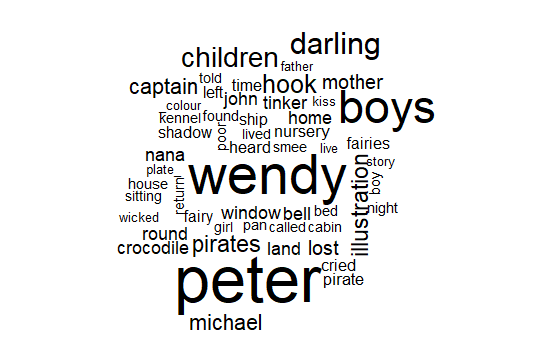
\includegraphics[scale=.5]{wordcloud}
\end{figure}

\end{frame}


\end{document}
